\documentclass{beamer}
\usepackage{siunitx}
\usepackage{tfrupee}
\let\vec\mathbf
\mode<presentation>
\usepackage{amsmath}
\usepackage{amssymb}
%\usepackage{advdate}
\usepackage{adjustbox}
%\usepackage{subcaption}
\usepackage{enumitem}
\usepackage{multicol}
\usepackage{mathtools}
\usepackage{listings}
\usepackage{url}
\usetheme{Boadilla}
\usecolortheme{lily}
\setbeamertemplate{footline}
{
  \leavevmode%
  \hbox{%
  \begin{beamercolorbox}[wd=\paperwidth,ht=2.25ex,dp=1ex,right]{author in head/foot}%
    \insertframenumber{} / \inserttotalframenumber\hspace*{2ex} 
  \end{beamercolorbox}}%
  \vskip0pt%
}
\setbeamertemplate{navigation symbols}{}
\providecommand{\nCr}[2]{\,^{#1}C_{#2}} % nCr
\providecommand{\nPr}[2]{\,^{#1}P_{#2}} % nPr
\providecommand{\mbf}{\mathbf}
\providecommand{\pr}[1]{\ensuremath{\Pr\left(#1\right)}}
\providecommand{\qfunc}[1]{\ensuremath{Q\left(#1\right)}}
\providecommand{\sbrak}[1]{\ensuremath{{}\left[#1\right]}}
\providecommand{\lsbrak}[1]{\ensuremath{{}\left[#1\right.}}
\providecommand{\rsbrak}[1]{\ensuremath{{}\left.#1\right]}}
\providecommand{\brak}[1]{\ensuremath{\left(#1\right)}}
\providecommand{\lbrak}[1]{\ensuremath{\left(#1\right.}}
\providecommand{\rbrak}[1]{\ensuremath{\left.#1\right)}}
\providecommand{\cbrak}[1]{\ensuremath{\left\{#1\right\}}}
\providecommand{\lcbrak}[1]{\ensuremath{\left\{#1\right.}}
\providecommand{\rcbrak}[1]{\ensuremath{\left.#1\right\}}}
\theoremstyle{remark}
\newtheorem{rem}{Remark}
\newcommand{\sgn}{\mathop{\mathrm{sgn}}}

\providecommand{\res}[1]{\Res\displaylimits_{#1}} 
\providecommand{\norm}[1]{\left\lVert#1\right\rVert}
\providecommand{\mtx}[1]{\mathbf{#1}}
\providecommand{\abs}[1]{\left\vert#1\right\vert}
\providecommand{\fourier}{\overset{\mathcal{F}}{ \rightleftharpoons}}
%\providecommand{\hilbert}{\overset{\mathcal{H}}{ \rightleftharpoons}}
\providecommand{\system}{\overset{\mathcal{H}}{ \longleftrightarrow}}
	%\newcommand{\solution}[2]{\textbf{Solution:}{#1}}
%\newcommand{\solution}{\noindent \textbf{Solution: }}align
\providecommand{\dec}[2]{\ensuremath{\overset{#1}{\underset{#2}{\gtrless}}}}
\newcommand{\myvec}[1]{\ensuremath{\begin{pmatrix}#1\end{pmatrix}}}

\title{Matrices in Geometry - 5.8.35}
\author{EE25BTECH11037  Divyansh}
\date{Sept, 2025}

\begin{document}

\maketitle


\section{Problem}
\begin{frame}
\frametitle{Problem Statement}
The cost of $4 \ kg$ onion, $3 \ kg$ wheat and $2\ kg$ rice is \rupee $60$. The cost of $2 \ kg$ onion, $4 \ kg$ wheat, and $6 \ kg$ rice is \rupee $90$. The cost of $6 \ kg$ onion, $2\ kg$ wheat, and $3\ kg$ rice is \rupee $70$. Find the cost of each item per kilogram.
\end{frame}

\section{Solution}
\begin{frame}{Solution}
   
Let the cost of 1 kg of onion, wheat and rice be \rupee $x$, \rupee $y$ and \rupee $z$, respectively.

The given information is:
\begin{align}
    \myvec{4 & 3 & 2}\myvec{x \\ y \\ z}=60 \\
    \myvec{2 & 4 & 6}\myvec{x \\ y \\ z}=90 \\
    \myvec{6 & 2 & 3}\myvec{x \\ y \\ z}=70 
\end{align}
Stacking them in a single matrix:
\begin{align}
    \myvec{4 & 3 & 2 \\ 2 &  4& 4 \\ 6 & 2 & 3}\myvec{x \\ y \\ z}=\myvec{60 \\ 90 \\ 70}
\end{align}
\end{frame}

\begin{frame}{Solution}
Writing the augmented matrix
\begin{align}
    \myvec{4 & 3 & 2 & \vrule & 60 \\ 2 &  4& 6 & \vrule & 90\\ 6 & 2 & 3& \vrule & 70}
    \overset{R_1 \rightarrow R_1 /4, R_2 \rightarrow R_2/2}{\longleftrightarrow}
    \myvec{1 & 3/4 & 1/2 & \vrule & 15 \\ 1 &  2& 3 & \vrule & 45\\ 6 & 2 & 3& \vrule & 70}\\
    \overset{R_2\rightarrow R_2-R_1, R_3 \rightarrow R_3 - 6R_1}{\longleftrightarrow}
    \myvec{1 & 3/4 & 1/2 & \vrule & 15 \\ 0 &  5/4& 5/2 & \vrule & 30\\ 0 & -5/2 & 0& \vrule & -20}\overset{R_2 \rightarrow 4R_2/5}{\longleftrightarrow}\\
     \myvec{1 & 3/4 & 1/2 & \vrule & 15 \\ 0 &  1& 2 & \vrule & 24\\ 0 & -5/2 & 0& \vrule & -20} \overset{R_1 \rightarrow R_1 - 3R_2/4, R_3 \rightarrow R_3 + 5R_2/2}{\longleftrightarrow}
\end{align}
\end{frame}

\begin{frame}{Solution}

\begin{align}
    \myvec{1 & 0 & -1 & \vrule & -3 \\ 0 &  1& 2 & \vrule & 24\\ 0 & 0 & 5& \vrule & 40}
    \overset{R_3 \rightarrow R_3/5}{\longleftrightarrow} \myvec{1 & 0 & -1 & \vrule & -3 \\ 0 &  1& 2 & \vrule & 24\\ 0 & 0 & 1& \vrule & 8}\\ \overset{R_1 \rightarrow R_1 + R_3, R_2 \rightarrow R_2 - 2R_3}{\longleftrightarrow}\myvec{1 & 0 & 0 & \vrule & 5 \\ 0 &  1& 0 & \vrule & 8\\ 0 & 0 & 1& \vrule & 8}
\end{align}

This implies that 
\begin{align}
    \myvec{x \\ y\\ z}=\myvec{5 \\ 8 \\ 8}
\end{align}
Therefore, the cost of 1 kg of onion, wheat, rice is \rupee $5$, \rupee $8$ and \rupee $8$.
\end{frame}
\begin{frame}{Solution}
    \begin{figure}[H]
        \centering
        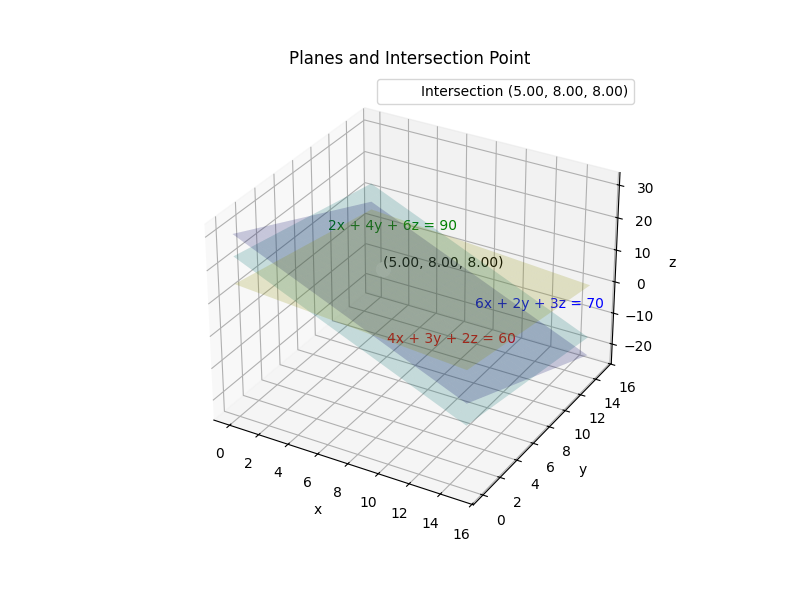
\includegraphics[width=0.7\columnwidth]{figs/1.png}
        \caption{Graph for 5.8.35}
        \label{fig:placeholder}
    \end{figure}
\end{frame}


\end{document}